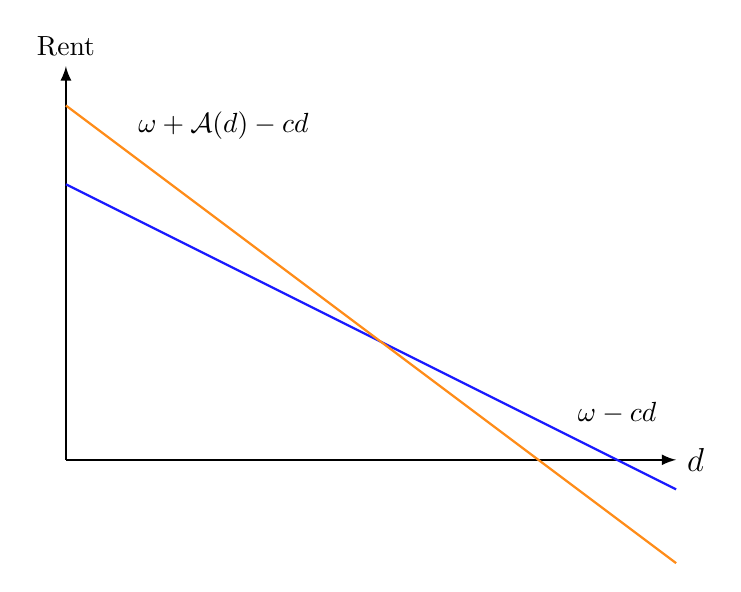
\begin{tikzpicture}[scale=.5]
\def\bndmax{5}        %https://tex.stackexchange.com/questions/68462/filling-a-complex-region-with-tikz
\def\bndmin{0.2}
\def \n {10}
\def \m {15.5}
\def \t {.5}
\def \th {1}
\def \w {7}
\tikzset{func/.style={thick,color=blue!90}}	
\draw [thick, latex-] (0,\n)node[above] {Rent}--(0,0);
\draw [thick, -latex] (0,0)--(\m,0)node[right=.25]{\large $d$};
%\foreach \xi in {0,..., \m} \draw (\xi,0)--(\xi,-.1)node[below=1]{\small$\xi$};
%\foreach \yi in {1,...,\n} \draw (0,\yi)--(-.1,\yi)node[left]{$\yi$};
%%\foreach \i in {1,4,9,16} {
	\draw[func,domain=0:\m] plot [samples=200] (\x,{\w-\t*\x});
%	\draw[func,domain=0:\m, dashed] plot [samples=200] (\x,{\w+\azero-\th*\x+\aprime*\x});

\node at (14,1.2){$\omega-cd$};
\def \azero{2}
\def \aprime {-.25}	
\tikzset{func/.style={thick,color=orange!90}}	
	\draw[func,domain=0:\m] plot [samples=200] (\x,{\w+\azero-\t*\x+\aprime*\x});
\node at (4,8.5){$\omega +\mathcal{A}(d)-cd$};
%\node at(-.8,2) [left]{base $2^1=$};
%\node at(-.8,1) [left]{$2^0=$};
%\draw[dotted] (0,2)--(1,2)--(1,0); 
 \end{tikzpicture}